\subsection{PCB Layout}
\label{sec:pcb-layout}

Careful consideration of the physical layout of the components on the printed circuit board (PCB) is important to reduce noise on the sensitive analog components.
Figure \ref{fig:layout} depicts the position of the components on the board.
Note the placement of the power electronics is away from the analog electronics and communications circuitry.

The PCB (figure \ref{fig:pcb-layout}) was designed in KiCAD.
The dimensions of the resulting board are $\SI{58}{\milli\metre}\times\SI{30}{\milli\metre}$, this is below the absolute maximum of $\SI{62}{\milli\metre}\times\SI{38}{\milli\metre}$.
\begin{figure}[H]
	\centering
	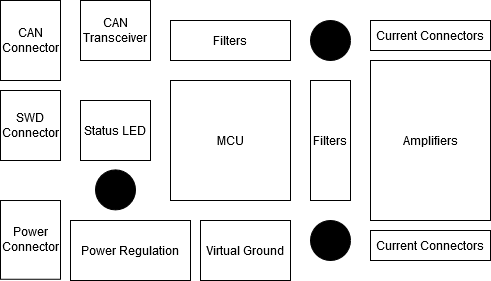
\includegraphics[width=0.8\textwidth]{layout}
	\caption{The approximate layout of the PCB.}
	\label{fig:layout}
\end{figure}

\begin{figure}[H]
	\centering
	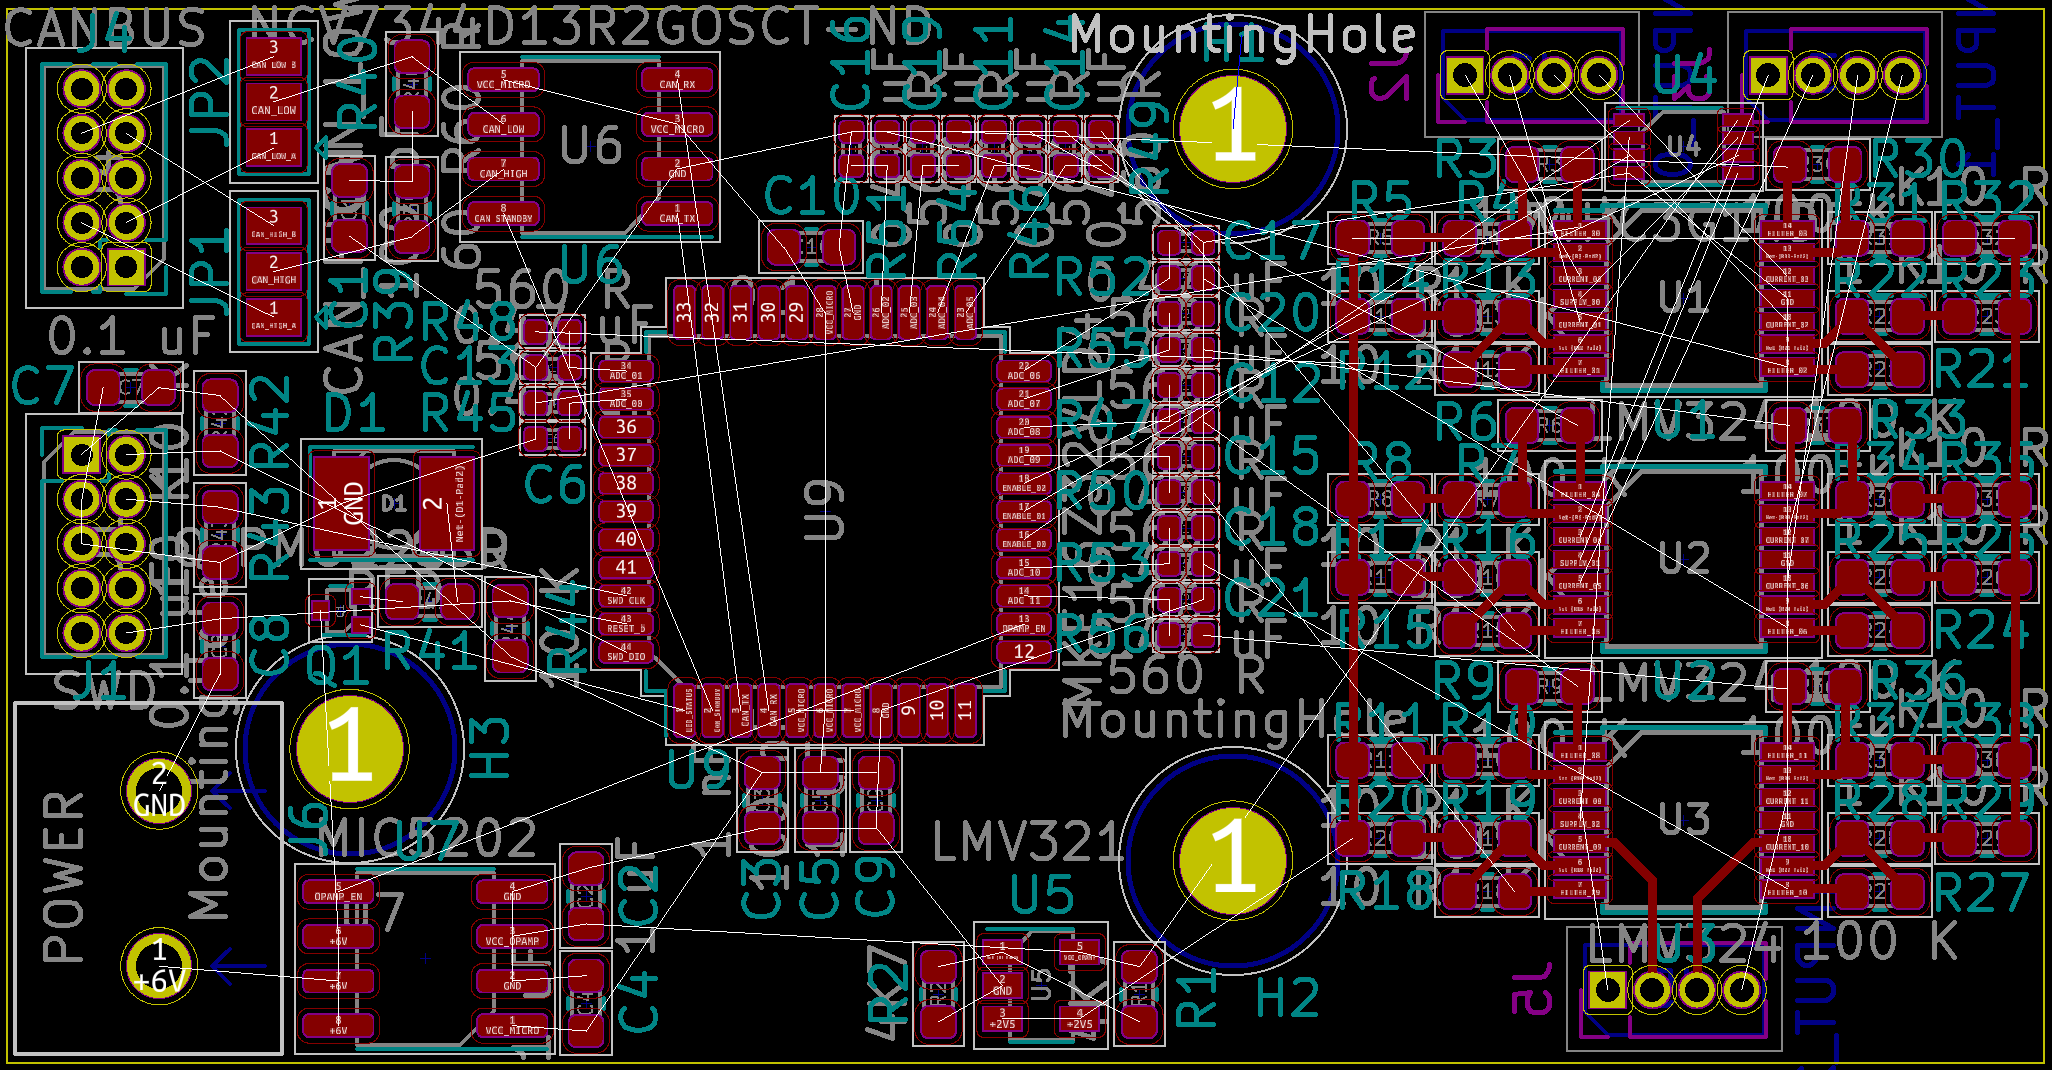
\includegraphics[width=\textwidth]{pcb_layout}
	\caption{The PCB layout viewed in KiCAD.}
	\label{fig:pcb-layout}
\end{figure}

% talk about the connectors to the motherboard
Three $\SI{2}{\milli\metre}$ diameter mounting holes are provided to aid in mounting the slave board on the motherboard.
The slave board would sit upon standoffs mounted to the motherboard using these mounting holes.
Three $\SI{1.27}{\milli\metre}$ pitch pin sockets connect the rear side of the PCB to the motherboard, either via short cables or a pin header arrangement.
The goal of this is to offer different mounting and connection options.
